\documentclass[A4]{article}
\usepackage{graphicx}
\usepackage[utf8]{inputenc}
\usepackage[backend=biber, style=iso-numeric, alldates=iso]{biblatex} % bibliografie
\usepackage[autostyle=true,czech=quotes]{csquotes}
\usepackage[czech]{babel}

\addbibresource{bibliography.bib}

\title{Analýza sítě Gnutella}
\author{Lukáš Moravec}
\date{\today}

\begin{document}

\begin{titlepage}
    \maketitle
\end{titlepage}
    
\section{Popis datové sady}
\cite{dataset} Datová sada byla získána ze \cite{snapnets} Standfordské velké kolekce datasetů. Jedná se P2P\footnote{Peer to peer}
síť pro sdílení souborů. Samotná datová sada obsahuje 8717 uzlů a 31525 orientovaných hran. Každý uzel reprezentuje účastníka připojeného
do sítě Gnutella a hrany reprezentují spojení mezi účastníky. Její kompletní znázornění lze vidět na obrázku \ref{network:full}.

\begin{figure}
    \centering
    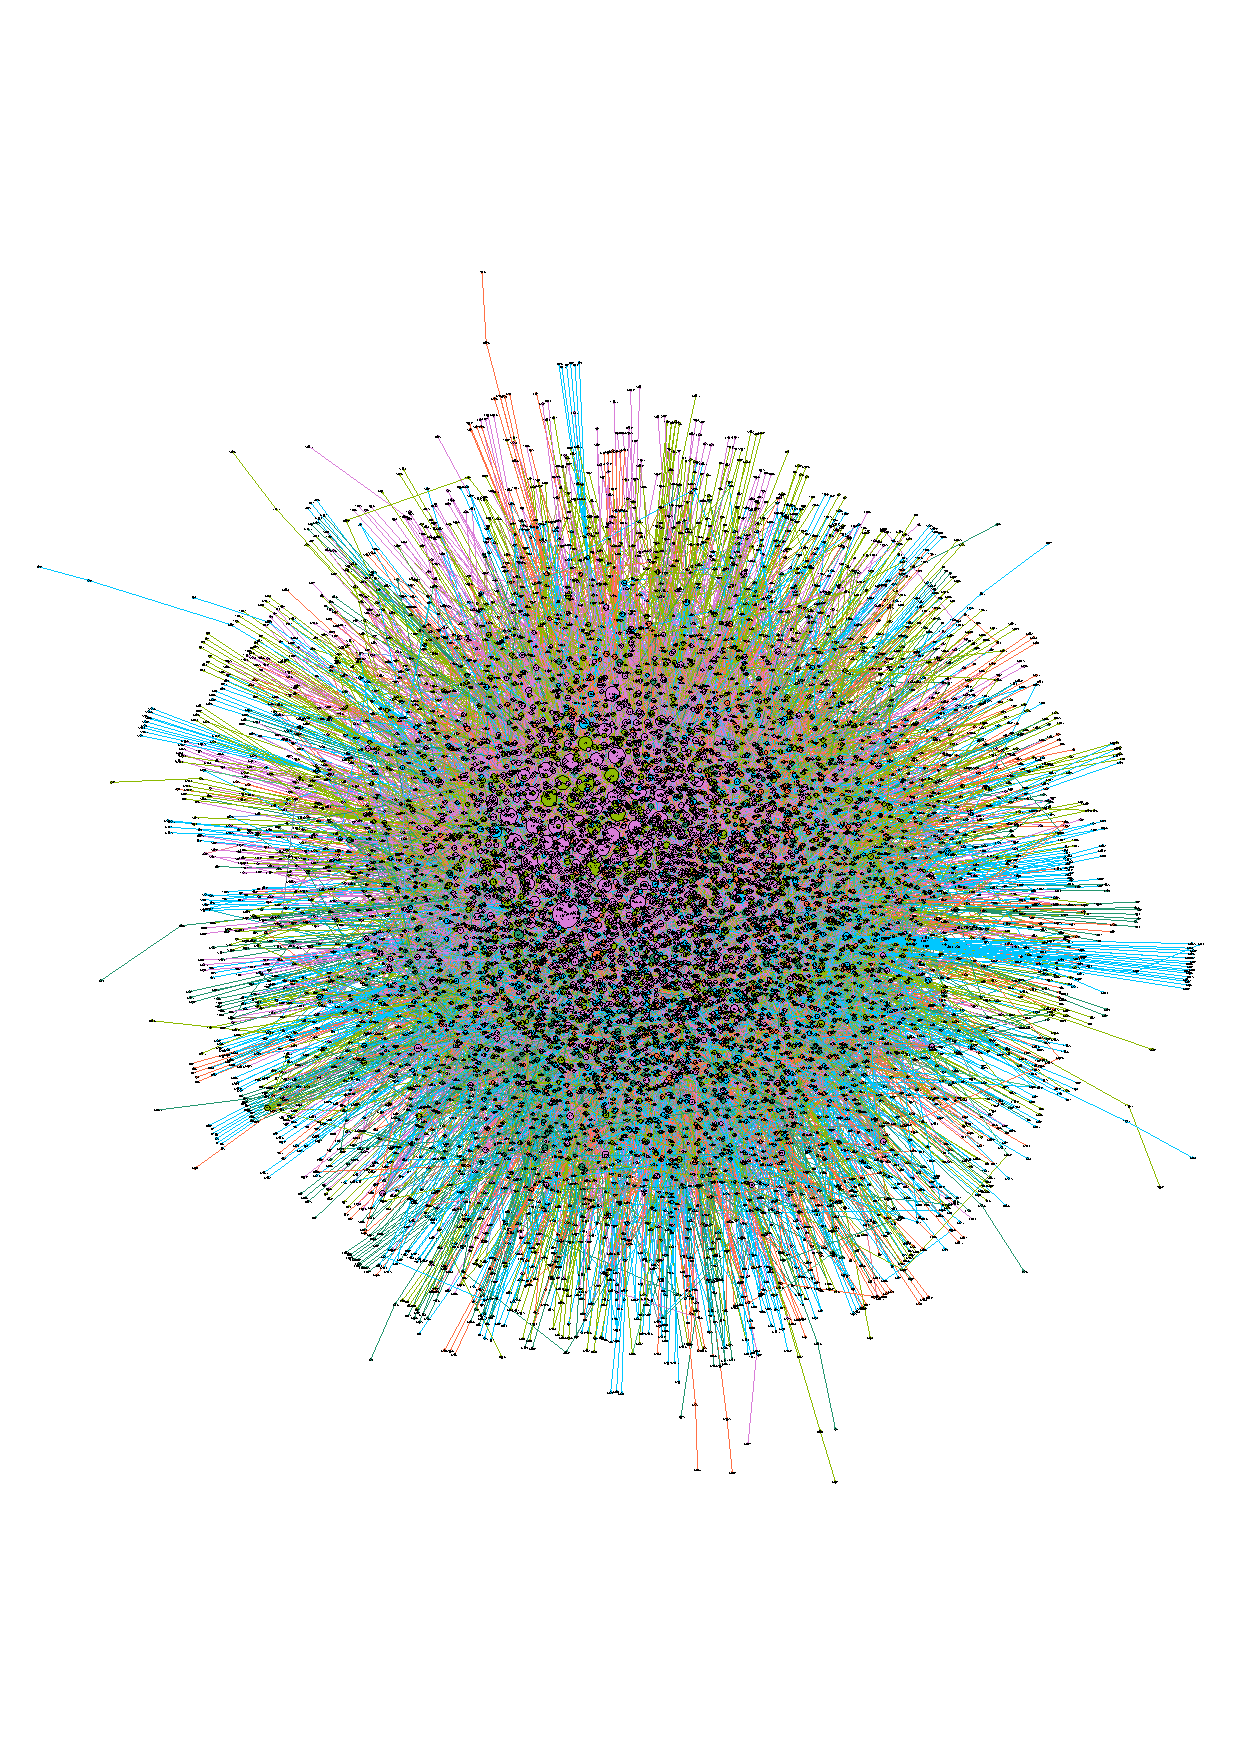
\includegraphics[width=1\textwidth]{export.pdf}
    \caption{Znázornění kompletní sítě}
    \label{network:full}
\end{figure}

\section{Statistiky}
K analýze sítě byl použit nástroj Gephi. Jelikož síť obsahuje velké množství uzlů, těžce se z ní na první pohled dá vyčíst něco zajímavého.
Proto jsem si uzly vyfiltroval podle stupňě uzlů > 15. Toto lze vidět na obrázku \ref{network:filtered}.

\begin{figure}
    \centering
    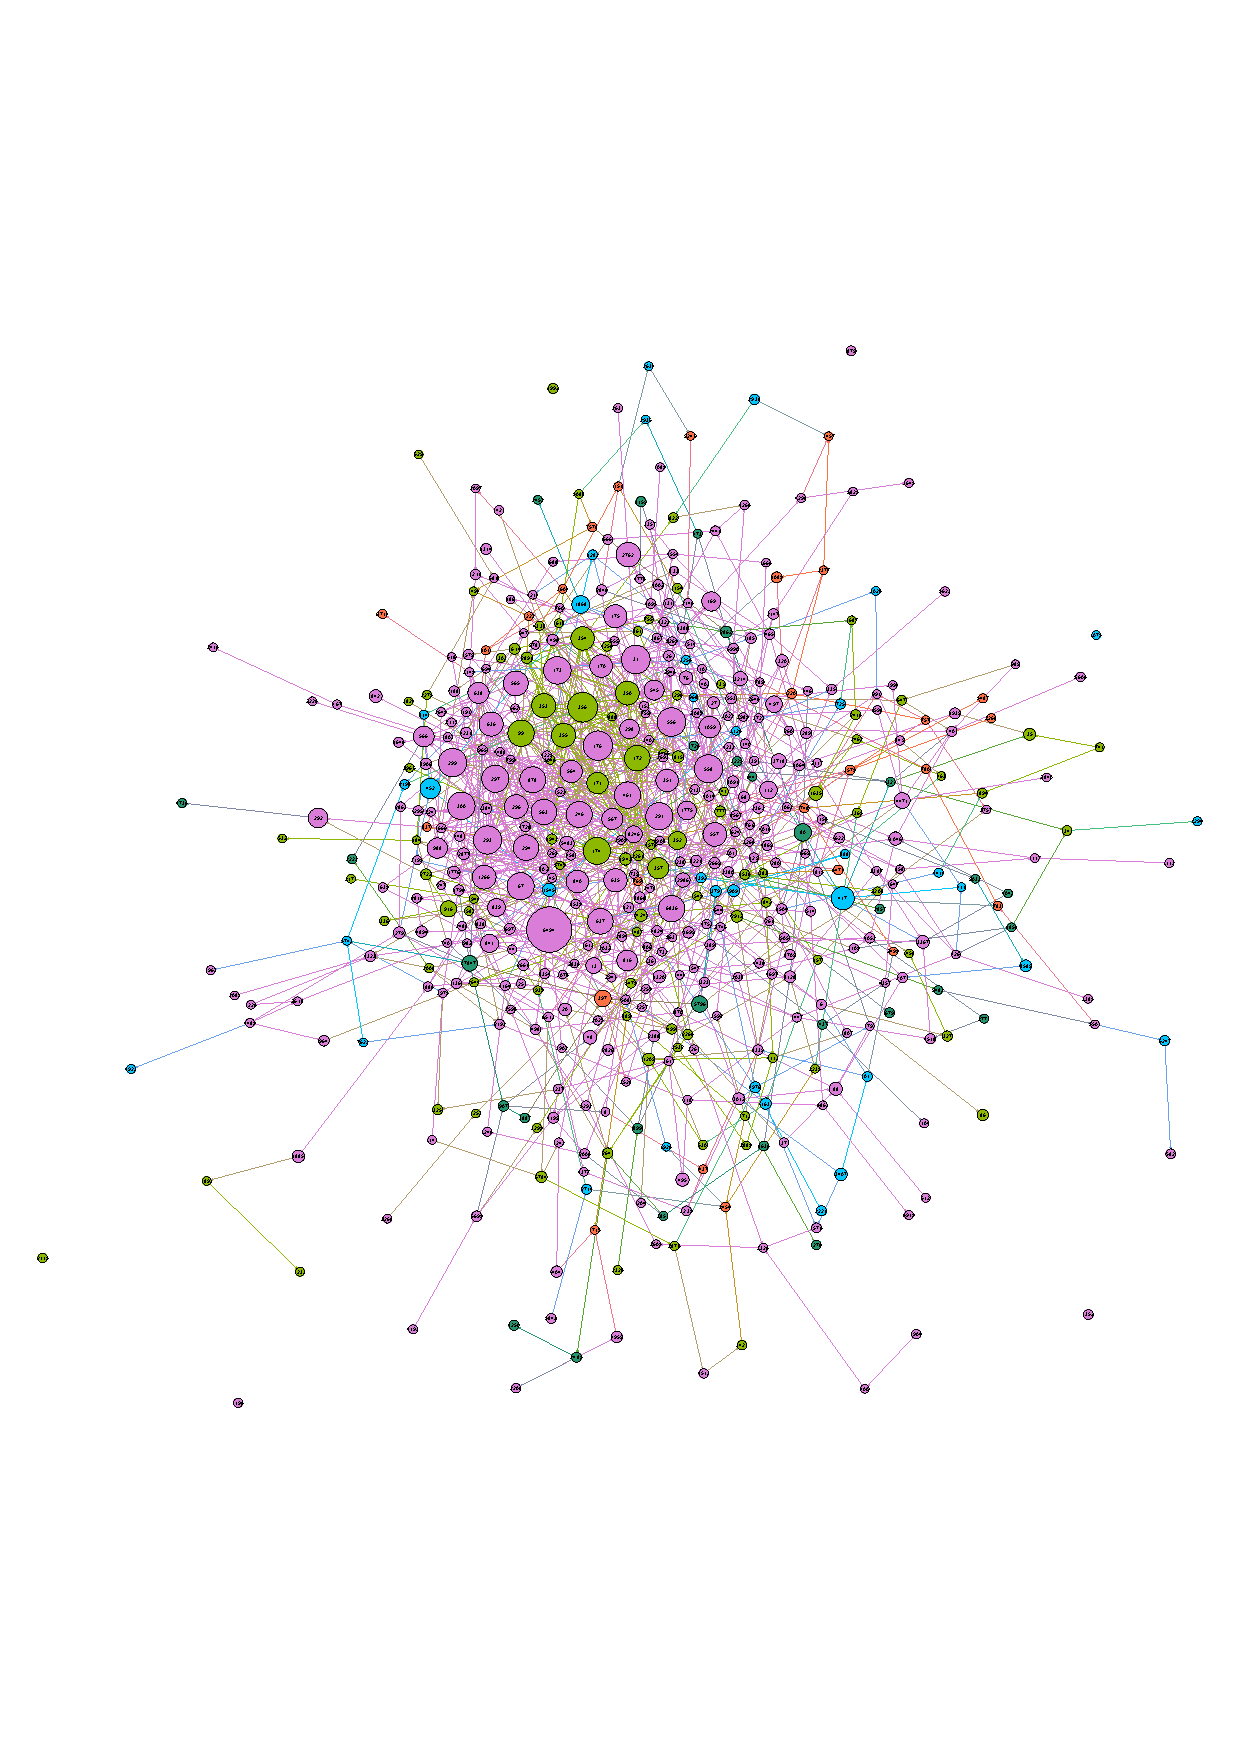
\includegraphics[width=0.7\textwidth]{export-filtered.pdf}
    \caption{Síť s vyfiltrovanými uzly se stupněm nižším než 15}
    \label{network:filtered}
\end{figure}

\clearpage
% Seznam literatury
\printbibliography[title={Literatura}, heading=bibintoc]
\end{document}
